The user evaluation cycle of Magpie was key in solidifying our target user base,
their wants \& needs as well as ensuring our application was user-friendly,
accessible and comprehensive.

The main takeaways from these in-depth sessions were:
\begin{itemize}
      \item \textbf{More data}: Majority of users, both domain and non-expert
            expressed their want for more amenity data on Magpie. This ranged from
            transportation data for route planning to a water grid overlay for town
            planners.
            
      \item \textbf{More features}: From the start of the user evaluation cycle
            with non-domain experts to the end, users have requested more features.
            Clear buttons were added, tooltips and a search functionality was
            implemented to the satisfaction of the users.
            
      \item \textbf{Improved visual feedback}: A key issue raised by users and
            also noted from their behaviour is more visual feedback when interacting
            with Magpie's control elements. Users want to see a reaction when pressing
            on the search, whether it was successful or not, and to interact with the tutorial.
\end{itemize}

Below is the summary of the UI scores from all the users interviewed.

%table summary ux scores users
\begin{figure}[htbp]
      \centering
      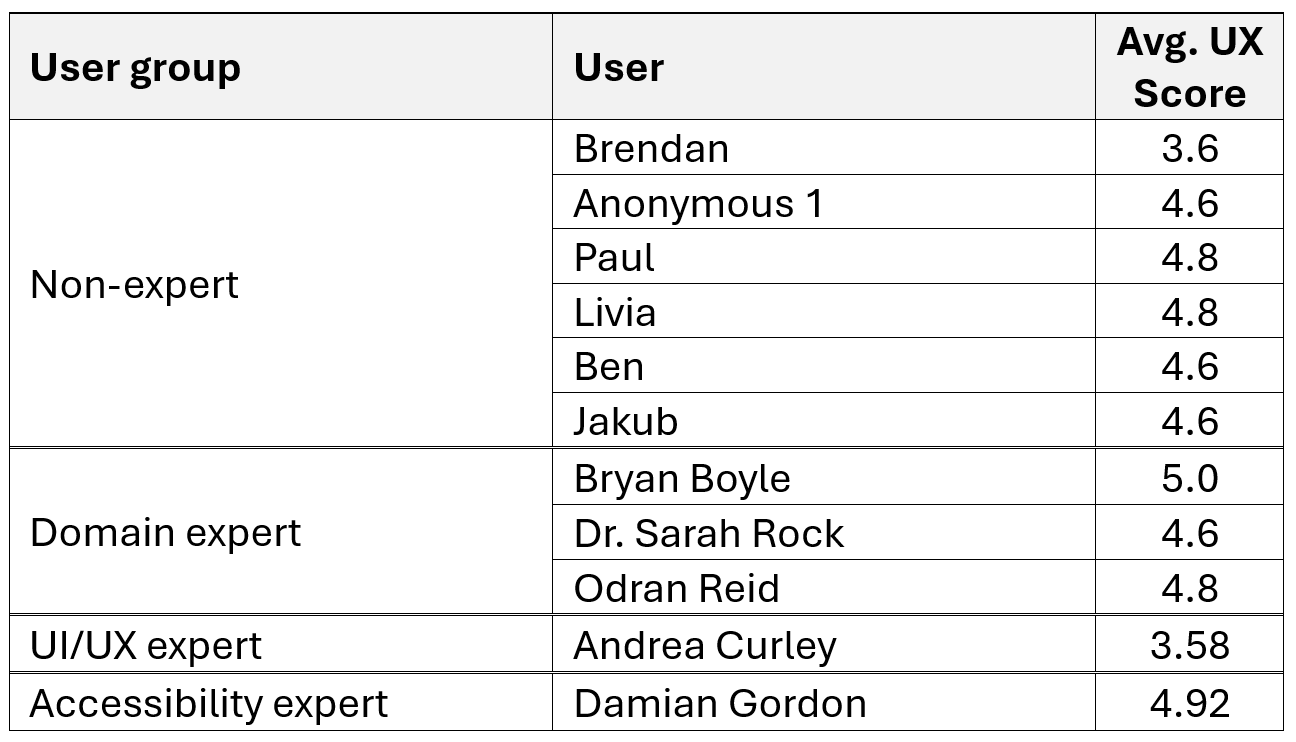
\includegraphics[width=0.8\textwidth]{images/ux-score-summary.png}
      \caption{UX score - Summary all users}
\end{figure}

There is still work to be done to improve the user flow of Magpie's interface,
as shown by the results from the UI/UX expert. However, the results from the
domain expert are extremely encouraging and validating to Magpie's core user goal of
providing a useful tool to planners.

\newpage{}